\linespread{1.3}
\chapter{Literature Review}
This chapter first defines the SED task, then introduces some sound event detection datasets which are popular in recent research literature, as well as the novel dataset used in the development of the SED system for this project. Next, it analyses different audio features, data augmentation techniques and sound event detection algorithms. From this analysis, this chapter then continues to identify issues with current SED research. 

\section{SED Definition}
SED is the task of recognising the sound events and their respective onset and offset timestamps in an audio clip recording. In real-life situations, sound events do not usually occur in isolation and are overlapped with one another. The task of detecting and recognising overlapped sound events is an extension of the typical SED task, and is known as polyphonic SED. For instance, speech, bird singing, and car passing by are detected in an audio clip, as shown in Figure \ref{fig:sed-system}. At certain timestamps, these sound events occur concurrently and overlap with one another, but have different onset and offset times. A general structure of a SED system is described in Figure \ref{fig:sed-structure}, which shows a waveform analysed in three main steps; feature extraction, frame-wise classification, and prediction post-processing. The purpose of the feature extraction step is to transform a waveform into a feature map that contains condensed information and is suitable for the subsequent stage of frame-wise classification, which predicts the probability of the presence of each sound event for each frame. A frame refers to a segment of the extracted features of the input waveform on the time axis. The last step involves processing of the frame-level class predictions, in which the onsets and offsets of the sound events are determined.

\begin{figure}[!htb]
    \centering
    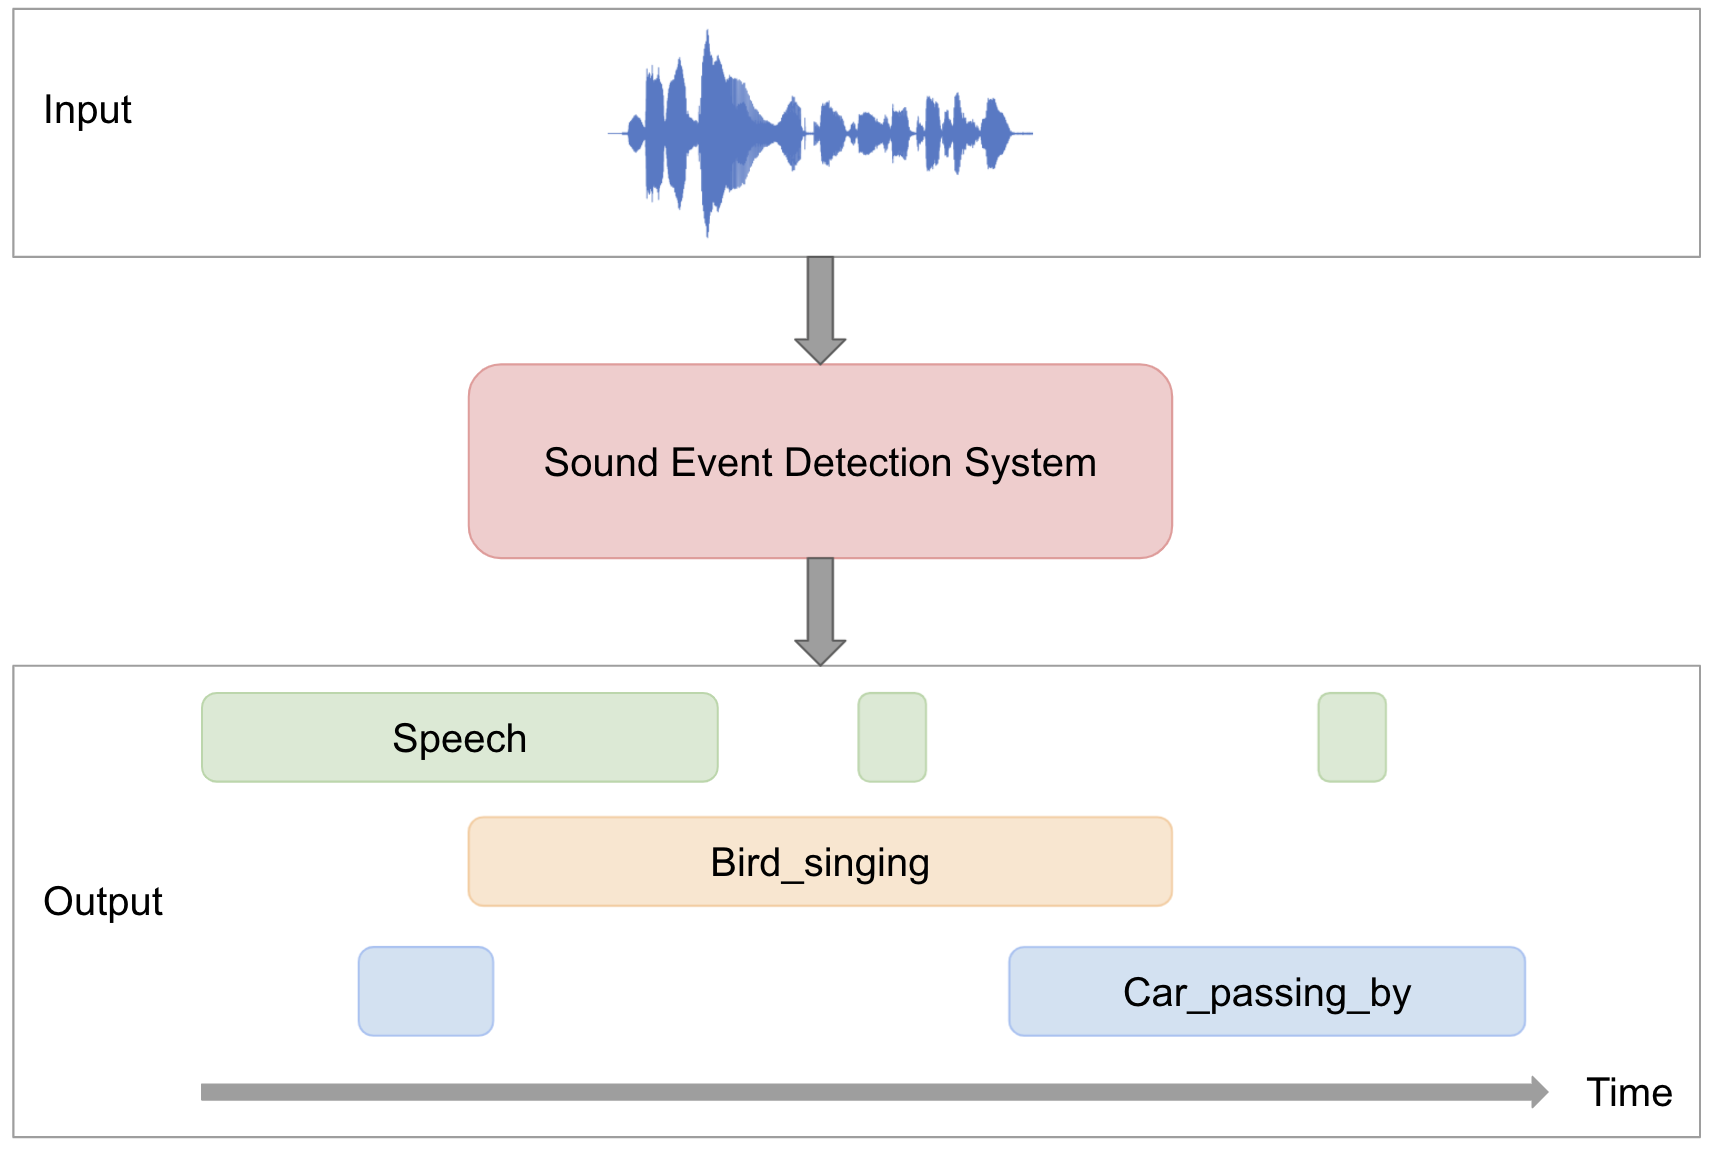
\includegraphics[width=\textwidth]{fig/sed-system.png}
    \caption{Overview of sound event detection system structure}
    \label{fig:sed-system}
\end{figure}

\begin{figure}[!htb]
    \centering
    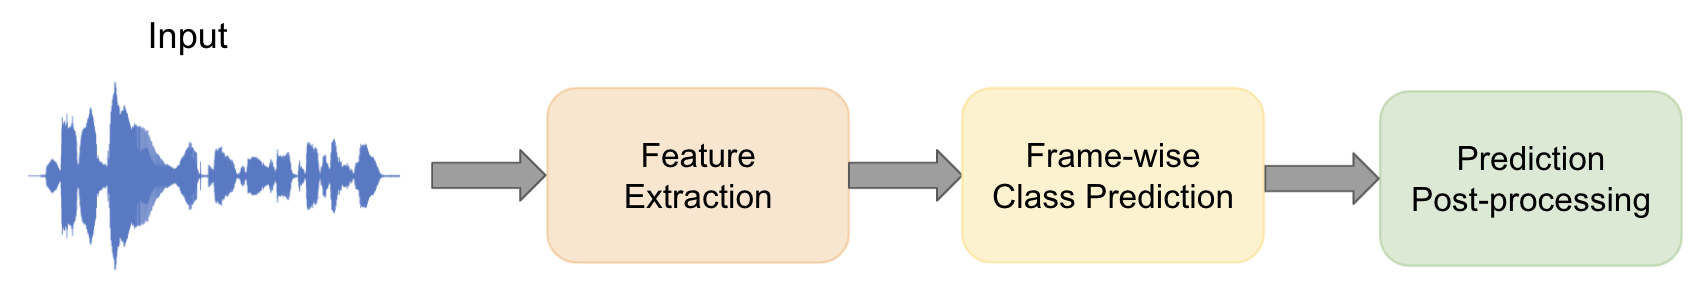
\includegraphics[width=\textwidth]{fig/sed-structure.png}
    \caption{Overview of sound event detection system}
    \label{fig:sed-structure}
\end{figure}

\section{SED Datasets}
This section introduces the common development datasets for SED tasks, as well as the novel dataset we curated for this project. Table \ref{tab:datasets} provides a summary of these datasets, most of which are from DCASE challenges. The audio clips in the DCASE datasets were recorded in real environments and released alongside the necessary meta information in WAV format.

\begin{table}[!htp]
\centering
\resizebox{\textwidth}{!}{\begin{tabular}{|c|c|c|c|c|c|c|c|}
\hline
\textbf{Dataset Name}                                                                                                                                       & \textbf{\begin{tabular}[c]{@{}c@{}}Year of \\ Release\end{tabular}}          & \textbf{\begin{tabular}[c]{@{}c@{}}Number \\ of Classes\end{tabular}} & \textbf{\begin{tabular}[c]{@{}c@{}}Total Audio\\ Duration\\ (Hours)\end{tabular}}     & \textbf{\begin{tabular}[c]{@{}c@{}}Segment\\ Length\\ (Seconds)\end{tabular}} & \textbf{\begin{tabular}[c]{@{}c@{}}Strongly\\ -labelled\end{tabular}}   & \textbf{\begin{tabular}[c]{@{}c@{}}Weakly\\ -labelled\end{tabular}}      & \textbf{Unlabelled}                                                    \\ \hline
\begin{tabular}[c]{@{}c@{}}DCASE 2020 Task 4\\ DCASE 2019 Task 4\\ DCASE 2018 Task 4\\ DCASE 2017 Task 4\\ DCASE 2016 Task 4\\ Project Dataset\end{tabular} & \begin{tabular}[c]{@{}c@{}}2020\\ 2019\\ 2018\\ 2017\\ 2016\\ -\end{tabular} & \begin{tabular}[c]{@{}c@{}}10\\ 10\\ 10\\ 17\\ 18\\ 25\end{tabular}   & \begin{tabular}[c]{@{}c@{}}51.59\\ 53.34\\ 45.22\\ 162.95\\ 1.88\\ 82.10\end{tabular} & \begin{tabular}[c]{@{}c@{}}10\\ 10\\ 10\\ 10\\ 10\\ 10\end{tabular}           & \begin{tabular}[c]{@{}c@{}}Yes\\ Yes\\ No\\ No\\ Yes\\ Yes\end{tabular} & \begin{tabular}[c]{@{}c@{}}Yes\\ Yes\\ Yes\\ Yes\\ No\\ Yes\end{tabular} & \begin{tabular}[c]{@{}c@{}}Yes\\ Yes\\ Yes\\ No\\ No\\ No\end{tabular} \\ \hline
\end{tabular}}
\caption{\label{tab:datasets}Sound event detection datasets}
\end{table}

 Most of these datasets, such as those from the DCASE 2017\cite{DCASE2017}, DCASE 2018 \cite{DCASE2018}, DCASE 2019 \cite{DCASE2019} and DCASE 2020 \cite{DCASE2019, Wisdom_InPrep2020} challenges, consist of a subset of the AudioSet dataset. AudioSet consists of 2,084,320 human-labelled 10-second audio clips extracted from YouTube videos and is made up of an ontology of 632 sound event classes  \cite{audioset}. There are two types of annotated data these datasets generally contain, namely strongly-labelled data and weakly-labelled data. The strongly-labelled data contains the specific onset and offset timestamps of when the sound events occur in a particular audio clip, while the weakly-labelled dataset only contains the tag information, which refers to the sound events that occur in a particular audio clip. Figure \ref{fig:weak-vs-strong} shows a comparison between strongly-labels and weakly-labels of an audio clip.\\

\begin{figure}[!htb]
    \centering
    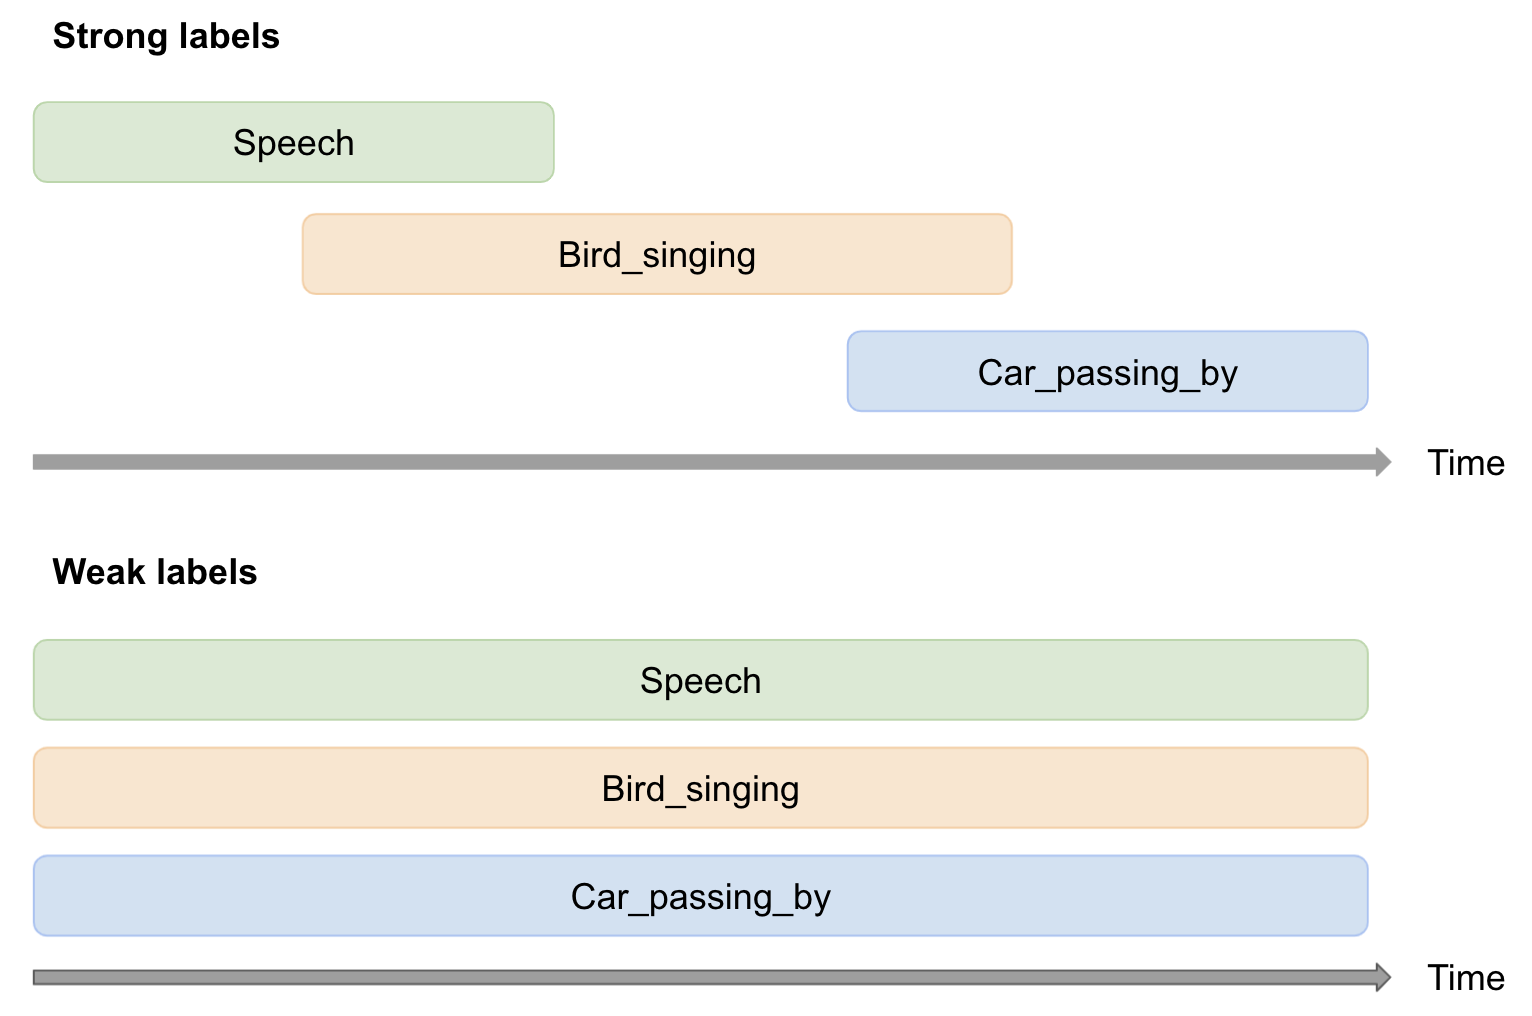
\includegraphics[width=\textwidth]{fig/weak-vs-strong.png}
    \caption{Comparison between strongly-labelled and weakly-labelled data}
    \label{fig:weak-vs-strong}
\end{figure}

% AudioSet is made up of an ontology of 632 audio event classes and a collection of 2,084,320 human-labelled 10-second sound clips extracted from YouTube videos \cite{audioset}. The ontology is a hierarchical graph of event categories which covers a wide range of human and animal sounds, musical instruments and genres, and everyday environmental sounds. The DCASE 2016 dataset \cite{DCASE2016} contains the highest number of sound event classes at 18, followed by DCASE 2017 \cite{DCASE2017} with 17 classes, then DCASE 2018 \cite{DCASE2018}, DCASE 2019 \cite{DCASE2019}  and DCASE 2020 \cite{DCASE2019, Wisdom_InPrep2020} with 10 classes. 
% The datasets also differ in terms of the types of data they contain. DCASE 2016 contains only strongly-labelled data while DCASE 2017 is only made up of weakly-labelled data. The remaining datasets contain a mix of data types. DCASE 2018 consists of unlabelled and weakly-labelled data while both DCASE 2019 and DCASE 2020 contain unlabelled, weakly-labelled and strongly-labelled data. 
% These DCASE challenges have provided a diverse set of sound event detection datasets and motivated many publications that have been evaluated with these datasets. 

In addition to these standard datasets provided by the DCASE challenges over the years, we have also curated our own dataset for this project in order to develop an SED system that is able to fulfil the requirements provided by our collaborating partner, DSO National Laboratories. The dataset is a subset of AudioSet \cite{audioset}, consisting of audio clips from 25 sound event classes related to human and emergency sounds, which is the highest number of sound event classes out of all the datasets discussed so far. The curation process and detailed information of this dataset will be discussed in Section 3.1. In this thesis, the SED system we developed is also evaluated with the DCASE 2017 dataset.

% The dataset is made up of a subset of the AudioSet dataset \cite{audioset}, focusing specifically on human sounds and emergency sounds, and incorporates the recently released strongly-labelled annotations for a subset of AudioSet \cite{hershey2021benefit}.

\section{Audio Features}
As the raw waveform data from audio clips cannot be understood by neural networks directly, feature extraction is needed to convert them into an understandable format. There are variety of audio feature types, most of which are spectrogram-based. However, no single feature type has yet proven complete superiority over the others for all SED tasks. A  spectrogram  is  a  visual  representation  of  the  spectrum  of  frequencies  of sound as they vary with time. These spectrogram representations have higher resolution and contain more information than general frame-based approaches \cite{spec-2019}, in terms of both temporal and frequency dimensions. This thesis focuses on the usage of log-mel and gammatone spectrogram representations. 

% These spectrograms are extracted from the audio clips and fed as input for training, instead of the raw audio clips themselves.

\subsection{Log-mel Spectrograms}
Log-mel spectrograms \cite{hershey2017cnn} are spectrogram representations that are derived from the classic spectrogram by applying a weighted average of the absolute values squared of the Short-Term Fourier Transform (STFT). They have been the most commonly used type of spectrogram representation in SED and Acoustic Scene Classification literature \cite{kong2020sound, Miyazaki2020CONFORMERBASEDSE, const_thres}, especially in conjunction with Convolutional Neural Networks (CNNs). It visualizes sounds on the Mel scale rather than the frequency domain, with log magnitude applied. The mel scale is a logarithmic transformation of a signal’s frequency. The basis of the idea of this transformation is that sounds of equal distance on the mel scale are perceived to be of equal distance to humans \cite{mel-scale}. This means that it is better able to mimic our own perception of sound. A mel spectrogram can be defined as:
\begin{equation}
MS_g(f)(b, v) = \sum_k|F(f \cdot T_bg)(k)|^2 \cdot \Lambda_v(k),
\end{equation}

where \(f\) represents the input signal, \(g\) is the window function for generating the spectrogram, and \(\Lambda_v\) is the mel-filters for \(v \in I = {1, . . . , K}\), where \(K\) is the chosen number of filters. The steps for computing log-mel spectrograms are as follows:
\begin{enumerate}
\item{Sample the input with Hann windows of \(x\) size, making hops of \(y\) size each time to sample the next window. The values of \(x\) and \(y\) are pre-defined.}
\item{Map each window from time domain to frequency domain by using the Fast Fourier Transform (FFT) algorithm.}
\item{Generate a mel scale by taking the entire frequency spectrum, and separating it into \(z\) bins evenly spaced frequencies. The mel scale values are calculated as follows:
\begin{equation}
    m = 2595 log_{10}(1 + \frac{f}{100})
\end{equation}}
\item{Generate the spectrograms by decomposing the magnitude of the signal into its components, corresponding to the frequencies in the Mel scale, for each window. }
\item{Apply the logarithmic conversion of the powers at each of the mel scale frequencies.}
\end{enumerate}

\subsection{Gammatone Spectrograms}
Gammatone spectrograms \cite{gammatone} are generated using gammatone filter-banks. Although they are not as commonly used as log-mel spectrograms, the gammatone filter have been designed to provide a closer approximation to the bandwidths of filters human auditory system \cite{slaney} and thus should provide an efficient representation. A Gammatone filter can be defined as:

\begin{equation}
g_{f_c}(t) = t^{N-1}exp(−2{\pi}tb(f_c)) cos(2πf_ct + {\phi})u(t),  
\end{equation}

where N represents the filter order, \(f_c\) is the filter center frequency in Hz, and \(\phi\) is the phase. \(u(t)\) is the unit step function which is \(u(t) = 1\) for \(t \geqslant 0\) and 0 otherwise. \(b(f_c)\) is the bandwidth of the filter. Empirical evidence has shown that \(N = 4\) provides a good match to the human auditory filter shape \cite{deliang}. The bandwidth of a gammatone filter used to model the human auditory system is generally chosen to be \(b(f_c) = 1.019 ERB(f_c) \approx 24.7(4.37f_c + 1)\). These filters are represented by an impulse response that is the product of a gamma distribution and sinusoidal tone. The impulse response of a 8 channel filter-bank is shown in Figure \ref{fig:impulse-frequency}(a) \cite{abdulla-gammatone}. The gammatone filter-bank is made up of a set of gammatone filters, which are channels with different centre frequencies. This is done to obtain a representation similar to a FFT-based spectrogram. An example of the frequency response of a 8 channel filter-bank is shown in Figure \ref{fig:impulse-frequency}(b) \cite{abdulla-gammatone}.\\

\begin{figure}[!htp]
    \centering
    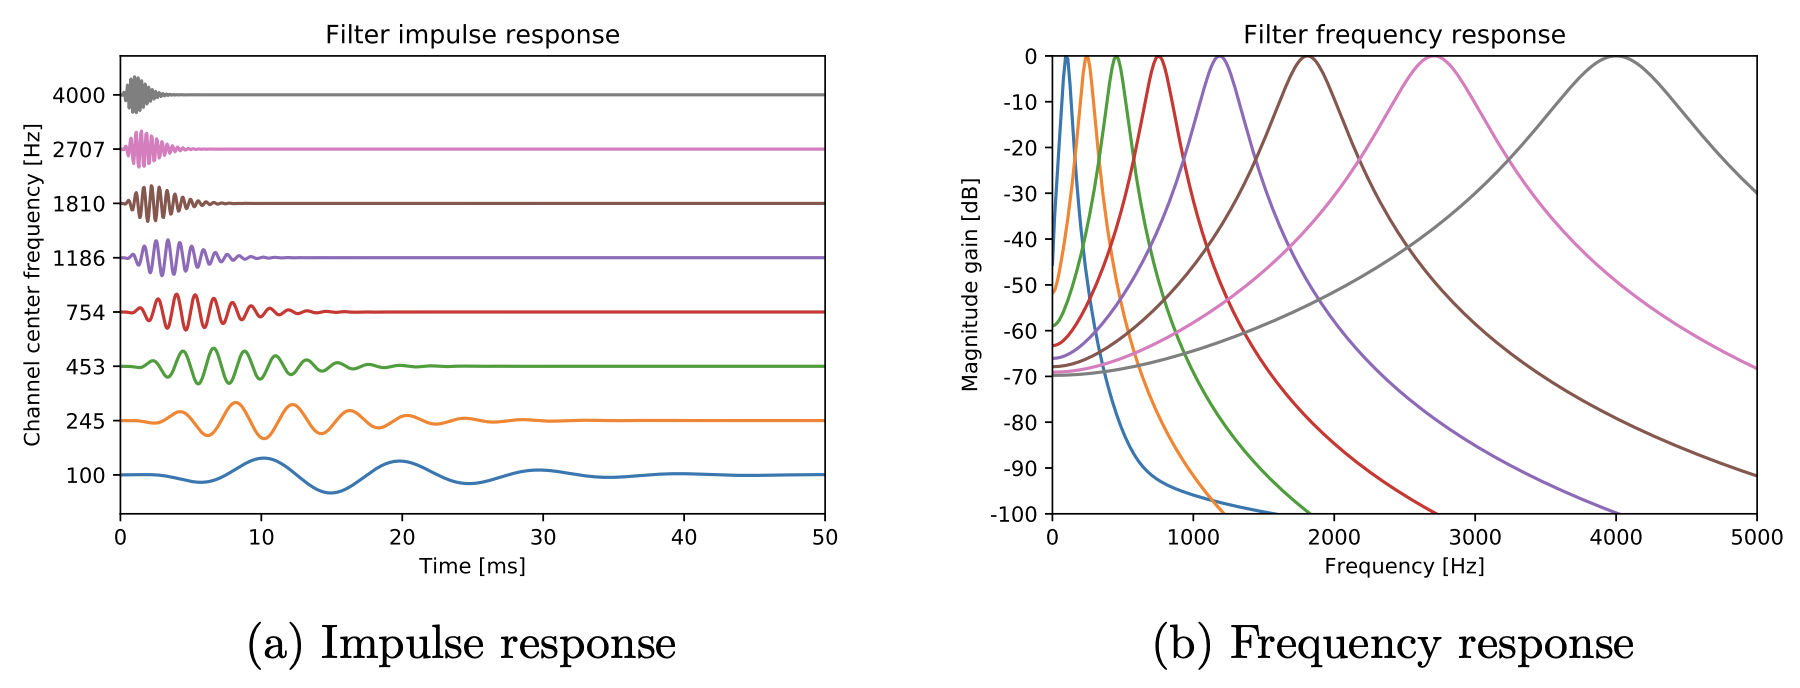
\includegraphics[width=\textwidth]{fig/impulse_frequency.png}
    \caption{Impulse (a) and frequency (b) response of a 8-channel filterbank, centered at equally spaced points between 100 Hz and 4 kHz
on the ERB scale}
    \label{fig:impulse-frequency}
\end{figure}

% \begin{figure}[!htb]
%     \centering
%     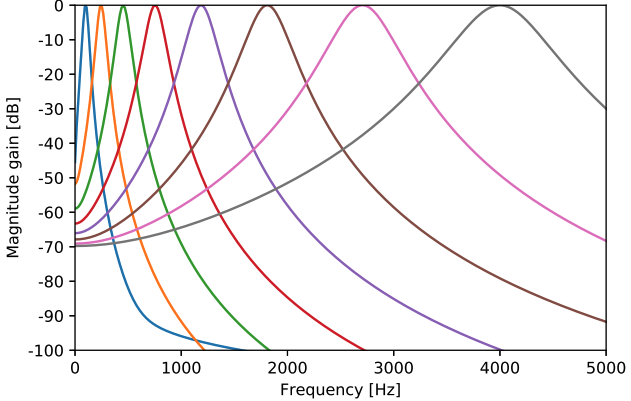
\includegraphics[width=0.7\textwidth]{fig/frequency-response.png}
%     \caption{Frequency response of a 8-channel filterbank, centered at equally spaced points between 100 Hz and 4 kHz
% on the ERB scale}
%     \label{fig:frequency-response}
% \end{figure}

% A set of gammatone filters, which are channels with different centre frequencies, is used to create the gammatone filter-bank. This is done to obtain a representation similar to a FFT-based spectrogram. An example of the frequency response of a 8 channel filter-bank is shown in Figure \ref{fig:frequency-response} \cite{abdulla-gammatone}.\\

The steps for computing gammatone spectrograms are as follows:

\begin{enumerate}
\item{Sample the input with Hann windows of \(x\) size, making hops of size \(y\) each time to sample the next window. The values of \(x\) and \(y\) are pre-defined.}
\item{Compute the Discrete Fourier Transform (DFT) for each window \(a^t\):
\begin{equation}
A^t_k = \sum^{n−1}_{m=0}a^t_m exp(−2{\pi}i\frac{mk}{n}), \quad k = 0, . . . , n - 1.
\end{equation}

The output of the DFT is Hermetian symmetric since the input windows are real-valued. Thus, the negative-frequency terms are redundant and can be removed. Since the first bin \(A^t_0\) contains the zero-frequency term of the signal, it is also removed. As a result, \(\frac{n}{2}\) points \(A^t = [A^t_1, A^t_2, ..., A^t_\frac{n}{2}]^T\) are left for each window.
\item{Compute the square of the absolute value of each window component. Stack the resulting vectors to obtain the power spectrogram A:
\begin{equation}
A = [|A^1|^2, |A^2|^2,  ..., |A^t|^2]
\end{equation}}
\item{Weight each bin \(|A^i|^2\) of the power spectrogram according to the expected magnitude gain of a gammatone filter of the same centre frequency corresponding to the DFT bin. This can be expressed by the matrix multiplication \(G = W A\). W is computed by transforming the impulse response of m gammatone filters evenly spaced on the ERB scale using an n-point DFT.
\begin{equation} W = 
\begin{bmatrix}
|DFT{g_{f1}(t)|^2\\
|DFT{g_{f2}(t)|^2\\
\vdots\\
|DFT{g_{fm}(t)|^2
\end{bmatrix}
\end{equation}}
\item{Apply the logarithmic conversion of the powers at each of the frequencies.}
\end{enumerate}

\section{Data Augmentation Techniques}
In the audio domain, data augmentation is used to artificially generate new data through data manipulation in order to improve generalisation and performance \cite{Wei_2020}. Although there are a variety of data augmentation techniques available, the authors Kong et al. \cite{kong2020sound} and Miyazaki et al. \cite{Miyazaki2020CONFORMERBASEDSE}, mainly focused on SpecAugment \cite{specaugment}, mixup \cite{mixup} and time-shift \cite{timeshift}, and managed to successfully produce the best-performing models for the DCASE 2017 and DCASE 2020 SED tasks respectively. As such, we will only focus on the aforementioned techniques in this thesis.

\subsection{SpecAugment}
Park et al. \cite{specaugment} developed SpecAugment to be used as a simple data augmentation technique for speech recognition tasks. The augmentation policy includes frequency-masking and time-masking. Figure \ref{fig:specaugment} shows a comparison between the original, frequency-masked, and time-masked audio.\\

\begin{figure}[!htb]
    \centering
    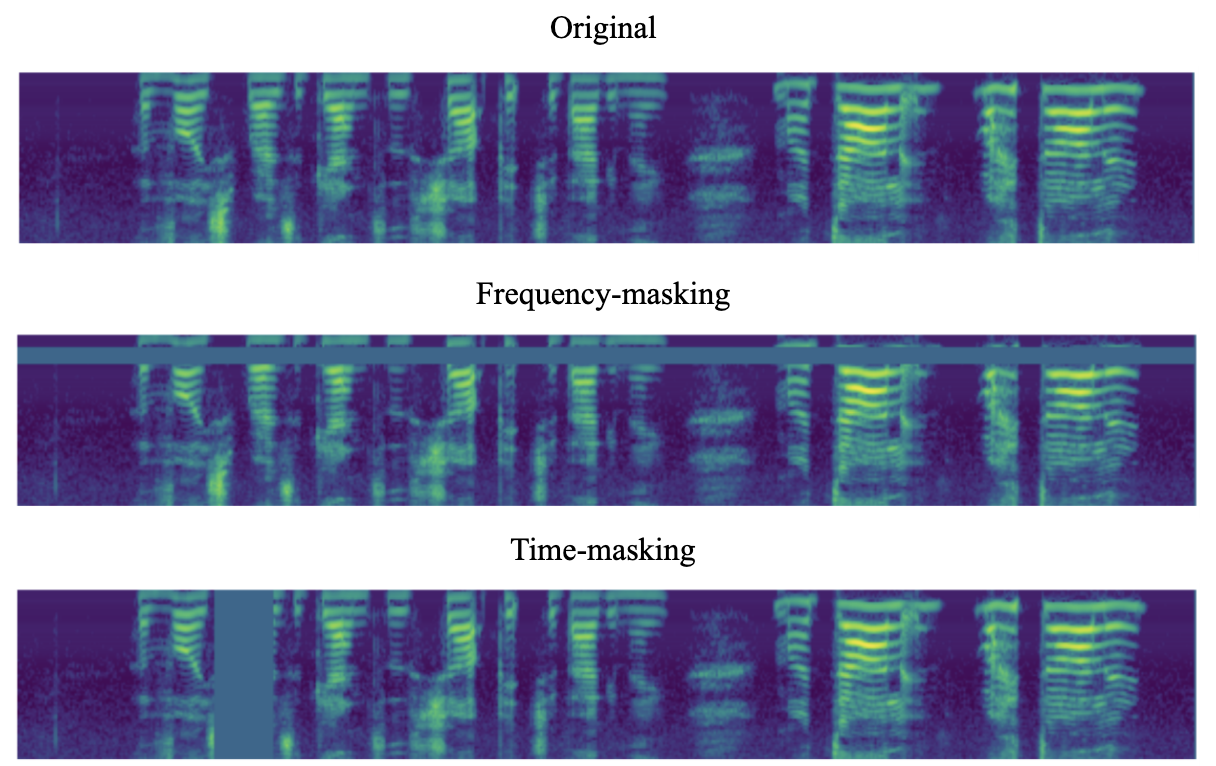
\includegraphics[width=\textwidth]{fig/specaugment.png}
    \caption{Comparison between original, frequency-masked and time-masked audio}
    \label{fig:specaugment}
\end{figure}

 In frequency masking, the frequency channels \([f_0, f_0 + f)\) are masked, which is done by replacing the corresponding values with zeroes. \(f\) is chosen from a uniform distribution between 0 and the frequency mask parameter \(F\), and \(f_0\) is chosen from \((0, v - f)\) where ν is the number of frequency channels. \\

Time masking replaces values in the time domain with zeroes, such that \(t\) consecutive time steps \([t_0, t_0 + t)\) are masked, where \(t\) is first chosen from a uniform distribution from 0 to the time mask parameter \(T\), and \(t_0\) is chosen from \([0, \tau - t)\), where \(\tau\) is the number of time steps.

\subsection{Mixup}
Zhang et al. \cite{mixup} originally developed mixup for computer vision tasks but its use has since been extended to the audio domain. Mixup smooths out the decision boundary by adding pseudo data generated by mixing different data points and the corresponding labels. By doing so, mixup regularizes the neural network to favour simple linear behavior in between training examples. Additionally, mixup has been found to decrease the memorization of corrupt labels, raise the robustness against adversarial examples, and stabilize the training of generative adversarial networks \cite{thulasidasan2020mixup}. Mixup can be represented in the following equation \ref{eqn:mixup-1} and \ref{eqn:mixup-2}:

\begin{align}
\label{eqn:mixup-1}
x¯ = \lambda{x_1} + (1 - \lambda)x_2,\\
\label{eqn:mixup-2}
y¯ = \lambda{y_1}+ (1 - \lambda)y_2,
\end{align}

where \((x_1, x_2)\) and \((y_1, y_2)\) represent different data points and their corresponding labels, respectively, and \(\lambda\) is the mixing \(\in\) [0,1]. In mixup, the \(\lambda\) value denotes the degree of mixing between the spectrograms. For instance, when mixup is applied on two spectrograms tagged with different sound events, the output spectrogram is a blend of the original two \cite{mixup_ex}. An example of mixup is shown in Figure \ref{fig:mixup}.

\begin{figure}[!htb]
    \centering
    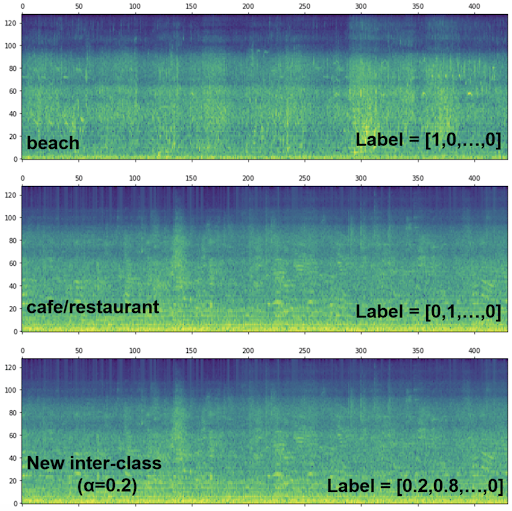
\includegraphics[width=0.8\textwidth]{fig/mixup.png}
    \caption{Example of mixup audio product}
    \label{fig:mixup}
\end{figure}

\subsection{Time-shift}
In time-shifting \cite{timeshift}, a feature sequence is shifted along the time axis, with the overrun frames being concatenated with the opposite end of the sequence. As reported in \cite{Miyazaki2020CONFORMERBASEDSE}, time-shifting has shown to help prevent the model from learning bias in time event localization. Figure \ref{fig:timeshift} shows a comparison between the original and time-shifted audio.

\begin{figure}[!htb]
    \centering
    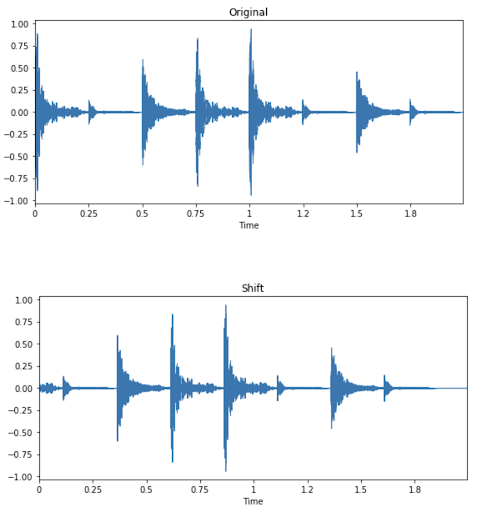
\includegraphics[width=0.8\textwidth]{fig/time-shift.png}
    \caption{Comparison between original and time-shifted audio}
    \label{fig:timeshift}
\end{figure}

\section{Deep Learning Approach}
The general approach to tackle the SED task is based on supervised learning, where a training set of audio recordings and their reference annotations of class events are used to learn an acoustic model. Early approaches for SED employed techniques from speech recognition and music information retrieval. These approaches were based on traditional pattern classification techniques such as Gaussian mixture models (GMMs) and hidden Markov models (HMMs). Notably, in 2007, Chien et al. \cite{Chien_2007} utilised GMMs for wheeze detection, and Schmidt et al. \cite{Schmidt_2010} employed HMMs to segment heart sound recordings in 2010. However, due to specific methods that allow the modelling of elementary units in speech or music, such as state-tying of phonemes or left-to-right topologies for modeling temporal evolution of phonemes and musical notes, GMMs and HMMs models are much more useful in speech and music modeling. Furthermore, sound events generally do not consist of similar elementary units as speech. This makes GMMs and HMMs less relevant for SED tasks. In addition, these models are not designed to detect multiple classes at the same time, making them unsuitable for polyphonic SED tasks. In order to solve the multi-label classification problem, they utilised extensions or setups, such as binary classification for each sound event class \cite{Mesaros2016TUTDF}, or multiple passes of Viterbi decoding \cite{heittola-2013} or pre-processing involving sound source separation \cite{heittola-2011}.\\ 

In contrast, modern pattern classification tools, especially deep neural networks (DNNs), can perform multi-label classification much more easily, as demonstrated by Cakir et al. \cite{Cakir_2015} in 2015. This is because multiple output neurons being active at the same time indicate the activity of multiple sound classes at the same time. This gives DNNs a great edge in solving the multi-label classification problem, and has made them predominant in the field. The utilisation of DNNs in SED tasks has allowed for major advancements in the field, with systems achieving state-of-the art performance and gaining the ability to tackle more complex problems.

\subsection{Convolutional Neural Network (CNN)}
CNNs were originally developed for image classification \cite{NIPS2012_cnn} but its usage has since been extended to audio related tasks such as sound event detection \cite{kong2020sound}, speech recognition \cite{cnn-asr} and audio tagging \cite{cnn-at}. Although we can construct an SED system purely from a CNN, its limited receptive field size means that it is unable to capture long time dependency in an audio clip. This is detrimental when analysing sound events that have long time dependencies. For example, a siren from an emergency vehicle may last for many seconds or even minutes. To allow the model to better capture the temporal dependency, Xu et al. \cite{xu2017convolutional} and Miyazaki et al. \cite{Miyazaki2020CONFORMERBASEDSE} have found that combining CNNs with other model types, such as RNNs, transformers and conformers allows the network to better extract the global and local context information from a feature sequence. This in turn makes for a better performing SED system.\\

A standard CNN comprises of convolution layers, pooling layers and fully connected layers. Each convolutional layer contains a set of learnable kernels, and its output is a tensor known as a feature map. These kernels are able to learn the local time-frequency patterns in the spectrogram extracted from an audio clip. In audio processing, the low level features \cite{thickstun2017learning} can be the raw wave-forms or spectrograms. The high level features are then extracted by the convolutional layers from these low level features. Following recent CNN architecures, batch normalization \cite{ioffe2015batch} is then applied after the convolutional layers to stabilise and increase the speed of training. After each batch normalization, non-linear activation functions, such as ReLU \cite{relu}, are then applied. For SED tasks, pooling layers are also applied along both time and frequency axes. Finally, the output of the last convolutional layer is fed as input to a time-distributed fully connected layer in order to predict the presence probability of sound events along the time axis. 

\subsection{Recurrent Neural Network (RNN) Based Models}
% As the receptive field of CNNs have limited sizes, this means that CNNs are unable to capture long time dependency in an audio clip. However, some sound events may have long time dependencies. For example, a siren from an emergency vehicle may last for many seconds or even minutes. In cases like these, temporal information would be especially useful for SED. Therefore, developing a system that is able to capture the temporal dependency, such as a CRNN \cite{xu2017convolutional}, is beneficial for SED tasks. 

Recurrent neural networks (RNNs) \cite{Mikolov:2010wx} are a type of neural network that can capture the long-term dependency of sequential data by storing history information in their hidden states. In fact, RNNs are frequently utilised in natural language processing tasks and have been shown to perform well in them \cite{devlin2019bert}. However, a possible problem with standard RNNs is that the gradient of the weights may vanish or explode during training. To prevent the gradient from exploding and vanishing, Long short term memory (LSTM) \cite{hochreiter1997long} systems have been developed. LSTMs are a variation of RNN and they comprise of constant error carousel units, input gate, output gate and forget gate. Notably, LSTMs have shown great promise in SED task, with Wang et.al \cite{Wang_2016} achieving better frame-wise performance through the use of it. LSTMs have also been further improved in the form of Gated Recurrent Units (GRUs) \cite{cho2014learning}. GRUs reduce the parameters of LSTMs and simplify the gates to a reset gate and a forget gate. Additionally, GRUs can be in both directions, which is known as a bidirectional GRU. In fact, Kong et al. \cite{kong2020sound} was able to achieve state-of-the-art performance for the DCASE 2017 SED challenge with the use of a bi-directional GRU, combined with a CNN, in his system. 
% Of the different variations of RNNs, we mainly experimented with the bi-directional GRUs in our thesis.

\subsection{Transformer-Based Models}
The transformer was originally proposed by Vaswani et al. \cite{vaswani2017attention} in 2017, and its design was motivated by the goal of allowing dependencies to be modelled without the consideration of their distance in the input sequence. In comparison to RNNs, the absence of recurrent connections in transformers allows for more parallel computing, which gives it slight advantage in terms of training speed. Transformers have mainly been applied in natural language processing tasks, but its use has since been extended to SED tasks, with good performance reported in \cite{kong2020sound}. However, Miyazaki et al. \cite{Miyazaki2020CONFORMERBASEDSE} has found that transformers are less effective in capturing local context information, which is essential for SED, in comparison to the more recently proposed Conformer model \cite{gulati2020conformer}.\\ 
 
A typical transformer may comprise of several encoder and decoder layers. When an input is fed into a transformer, it is transformed into a high level embedding by the encode, which can then be transformed to an output by the decoder. In SED tasks, only the encoder is required, and each encoder is made up several encoder layers. The encoder layer contains a query transform matrix \(W^Q\), a key transform matrix \(W^K\) and a value transform matrix \(W^V\). The matrices \(W^Q\) and \(W^K\) have a shape of \(C × d_k\), and \(W^V\) has a shape of \(C \times d_v\), where \(C\) represents the number of channels, and \(d_k\) and \(d_v\) are integers. Then the query \(Q\),  key \(K\) and value \(V\) can be obtained by:

\begin{align}
Q = xW^Q\\
K = xW^K\\
V = xW^V 
\end{align}

The query Q and key K have a shape of \(T \times d_k\), and the value \(V\) has a shape of \(T \times d_v\), where \(T\) refers to the number of time steps. The output of an encoder layer can be written as: 

\begin{equation}
\label{eqn:trans-4}
h = softmax(\frac{QK^T}{\sqrt{d_k}})V ,
\end{equation}

where the output \(h\) has a shape of \(T \times H\). In equation \ref{eqn:trans-4}, the division of the square root of \(d_k\) is a normalization term \cite{vaswani2017attention}, and the inner product of \(Q\) and \(K^T\) has a shape of \(T \times T\), which represents the feature correlation of different time steps. The softmax function transforms the correlation value to probabilities along the time steps, which indicate how much the value \(V\) in a time step should be attended to.

\subsection{Conformer-Based Models}
The conformer was originally proposed by Gulati et al. \cite{gulati2020conformer} in 2020. It is essentially a convolution-augmented Transformer. By combining self-attention with a CNN, it is able to achieve high performance and efficient parameter reduction. This is possible because it is able exploit the strengths of each component, that is, self-attention is better at modeling long-range, global context information, while CNNs are better at extracting local features. The conformer has been reported to achieve state-of-the-art performance in automatic speech recognition (ASR) and SED. Specifically, Miyazaki et al. \cite{Miyazaki2020CONFORMERBASEDSE} was able achieve the best-performing model for the DCASE 2020 Task 4 with the use of conformers in his system, with it slightly outperforming the transformer system he tested in his study as well.\\

The conformer block is made up of three modules, namely a feed-forward module, a multi-head self-attention module, and a convolution module. The feed-forward module comprises of a layer-normalization layer, a linear layer with a Swish activation function \cite{ramachandran2017searching}, which expands the dimensions of the input by four times, and finally another linear layer, which projects the dimensions back to those of the original input. The multi-head self-attention module contains a layer-normalization and multi-head self-attention with relative positional embedding, as used in Transformer-XL \cite{dai-etal-2019-transformer}. The convolution module is made up of a layer normalization layer, a point-wise convolution layer with a gated linear unit (GLU) activation function \cite{dauphin2017language}, and a 1-D depth-wise convolution layer, which is then followed by a batch normalization layer, Swish activation, and finally a point-wise convolution layer. The relation between the input \(X\) and output \(Y\) of the conformer block can thus be modelled as follows:

\begin{align}
X˜ = X + \frac{1}{2}FFN(X),\\
X` = X˜ + MHSA(X˜),\\
X`` = X` + Conv(X),\\
Y = LayerNorm(X`` + \frac{1}{2}FFN(X``)),  
\end{align}

where \(FFN(\cdot)\), \(MHSA(\cdot)\), \(Conv(\cdot)\), and \(LayerNorm(\cdot)\) refer to the feed-forward module, multi-head self-attention module, convolution module, and layer-normalization layer, respectively.

\subsection{Transfer Learning}
% % Transfer learning is a machine learning method where a model developed for a particular task is reused as the starting point for a model on a second task \cite{trans-learn}. With transfer learning, we can train a deep neural network with comparatively little data. 

In transfer learning, the knowledge of a pre-trained model is applied to a different but related problem \cite{trans-learn}. This is done to exploit what has been learned in one task to improve the generalisation of another. As such, transfer learning has the potential to speed up training and improve the performance of a neural network model. In fact, Jung et al. \cite{Jung_2019} reported a significant improvement in the performance of his SED system through the integration of transfer learning with his model.\\ 
% % In deep learning we transfer weights that a network has learned in one task to another. If the source and target data are similar, then the knowledge can be transferred from a high number of source layers. We will be exploring the use of transfer learning methods for CNN as it has proven to be useful \cite{trans-learn-2019}.\\ 

There are two main transfer learning strategies that can be applied, which are summaried in Figure \ref{fig:transfer-learning}. The first strategy is to use the pre-trained model as a feature extractor, with no further training done. In the context of the SED task, this means that the embedding features of audio clips are first calculated with the pre-trained model. These embedding features are later used as input to a classifier. When training on the new dataset, the parameters of the pre-trained model are frozen and not trained, and only the parameters of classifier built on embedding features are trained. This strategy is typically only used when the new dataset and the dataset the model was pre-trained on are similar. In contrast, the second strategy is to fine-tune the pre-trained model with the data from the new task. This involves initialising all the parameters from the pre-trained model, except final fully-connected layer. These parameters are then further trained on the dataset of the new task.

\begin{figure}[!htp]
    \centering
    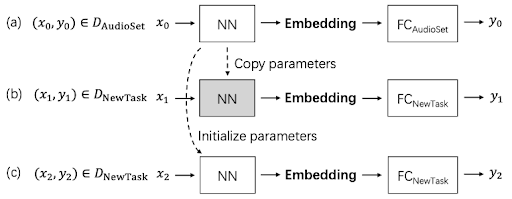
\includegraphics[width=\textwidth]{fig/transfer-learning.png}
    \caption{Transfer learning strategies. (a) represents the pre-trained model. (b) is the pre-trained model being using as a feature extractor. (c) is where the pre-trained model is fine-tuned on the new dataset.}
    \label{fig:transfer-learning}
\end{figure}

\section{Automatic Threshold Optimisation}
The threshold values play an important role in prediction post-processing in SED tasks. That is, if the predicted probability that a certain sound event is present in a frame exceeds the threshold value, then the frame is regarded to contain this sound event. The selection of the threshold values for post-processing is a challenging problem. They are typically manually selected, and are commonly set to 0.5 for most SED systems \cite{const_thres}. However, these threshold values are usually not optimal for all the sound event classes. As such, the selection of threshold values is an important part of SED tasks as incorrect selection may have detrimental effects on the performance of a SED system. In order to solve this problem, Kong et al. \cite{kong2020sound} has proposed an automatic threshold optimisation method to determine the optimal threshold values for different sound event classes. The automatic threshold optimisation method optimises thresholds based on a metric such as F1-score, and  has been found to improve the performance of SED systems. Hence, we will be experimenting with the use of automatic threshold optimisation in this thesis since it has been proven to be useful in similar tasks.

\section{Open Issues}
Existing literature on SED, specifically for the recent DCASE SED challenges, have mainly developed systems to analyse audio clips as a whole and have yet to explore the impacts of applying rolling segmentation windows on the audio clips prior to analysis. This is in spite of the fact that doing so may yield potential benefits, especially in real-life applications. In real-life applications, the audio clips we would usually like to analyse could be hours long. Therefore, processing these long audio clips as a whole is not feasible as it is online and on the fly. As such, they are usually divided into segments of \(x\) seconds and fed into the system for analysis. However, just purely dividing the audio clips into non-overlapping segments and sending them for analysis may not yield the best outcome. This is because depending on the segment length or the temporal position where the audio clip is partitioned and sent to the system for analysis, the SED system may output slightly different results. For edge cases, such as sound events occurring right at the end of one segment and continuing over to the succeeding segment, the SED system may not even be able to detect them as the sound event is broken apart and not analysed as a whole. In this thesis, we will explore this issue and propose some methods, such as averaging frame-wise predictions, to remedy it.

% Existing literature on SED have only focused on developing systems to have optimised performance on the common SED datasets mentioned in Section 2.2, whose evaluation sets only consist of 10 second long audio clips, and have overlooked optimising their performance on clips with long audio duration. However, in real-life applications, the audio clips we would usually like to evaluate on could be hours long. Processing these long audio clips as a whole is not feasible as it is online and on the fly. Therefore, they are usually divided into segments of \(x\) seconds and fed into the system for analysis. Depending on the segment length or the temporal position where the audio clip is portioned and sent to the system for analysis, the SED system may output slightly different results. For edge cases, such as sound events occurring right at the end of one segment and continuing over to the succeeding segment, the SED system may not even be able to detect them as the sound event is broken apart and not analysed as a whole. In this thesis, we will explore this issue and propose some methods, such as averaging frame-wise predictions, to remedy it.

% The issues of how an audio clip recording should be segmented before being sent to the SED system to be analysed, and how it should be processed after, is often overlooked in scientific publications. This is especially important when analysing clips with long audio durations.  


%=== END OF LITERATURE REVIEW ===
\newpage